\documentclass{PHlab-thesis}

\addbibresource{thesis.bib}

\newcommand*\Department中文{資訊工程學研究所}
\newcommand*\Department英文{Institute of Computer Science and Information Engineering}

\newcommand*\ThesisTitle中文{使用深度強化學習提升物件偵測性能}
\newcommand*\ThesisTitle英文{Deep Reinforcement Learning for Enhancing Object Detection Performance}
\newcommand*\ThesisNote中文{示例:其實徐翡曼是東京大學畢業的博士}% For real thesis omit, or use {初稿} etc.
\newcommand*\ThesisNote英文{Just an example.  Fei-Man actually graduated from Tokyo Univ.}% For real thesis omit, or use {draft} etc.

\newcommand*\Student中文{郭育丞}
\newcommand*\Student英文{Yu-Cheng Guo}

\newcommand*\Advisor中文{賀保羅}
\newcommand*\Advisor英文{Paul Horton}

%% 果有共同指導老師可以用:
%% \newcommand*\CoAdvisorA中文{}
%% \newcommand*\CoAdvisorA英文{}
%% \newcommand*\CoAdvisorB中文{}
%% \newcommand*\CoAdvisorB英文{}


\newcommand*\YearMonth英文{July, 2023}
\newcommand*\YearMonth中文{一一二年七月}

\usepackage{float}
\usepackage{enumerate}
\usepackage{graphicx}
\usepackage{subfigure}
\usepackage{caption}
\graphicspath{ {./images/} }

\fancyhead[L]{\small\leftmark}
\fancyhead[R]{\small\rightmark}
\pagestyle{fancy}% Use fancyhdr
\begin{document}


\newcommand*\Keywords英文{Deep reinforcement learning, Object detection}
\newcommand*\Abstract英文{%
In recent years, deep learning techniques have made significant progress in the field of image processing and analysis, especially in the area of object detection. However, the performance of trained object detection neural networks depends largely on the image quality, and it is still a challenging problem to improve the detection accuracy. Image quality can be affected by a variety of factors, such as blurred images, noise, low contrast, insufficient lighting, or overexposure. These problems may make it difficult for deep learning models to accurately identify and localize objects. To overcome these challenges, this study proposes a method to achieve enhanced object detection using deep reinforcement learning DDPG as well as YOLOv7. In this approach, we use pre-processing techniques for image saturation, brightness, contrast, and sharpness to improve image quality. These pre-processing steps are performed by the DDPG algorithm to further enhance the image. Then, we use the pre-processed images as input to YOLOv7 to achieve better object detection. Our experimental results show that this new object detection method achieves better detection accuracy than using only YOLOv7 alone.
}


\newcommand*\Keywords中文{深度強化學習、物件偵測}
\newcommand*\Abstract中文{%
近年來,深度學習技術在影像處理和分析領域中取得了顯著的進展,尤其在物件偵測方面,取得了顯著的成果。然而,經過訓練的物件偵測神經網路的性能在很大程度上取決於影像品質,如何提高偵測的精度仍然是一個具有挑戰性的問題。影像品質可能受到多種因素的影響,例如圖像模糊、噪音、低對比度、光照不足或過度曝光等。這些問題可能導致深度學習模型難以準確地識別和定位物件。為了克服這些挑戰,本研究提出了一種方法,使用深度強化學習 DDPG 以及 YOLOv7 來實現增強物件偵測的效果。在這種方法中,我們使用前處理技術對影像進行飽和度、亮度、對比度和銳利度處理,以提高影像品質。這些前處理步驟由 DDPG 算法負責執行,以進一步增強影像。接著,我們將經過前處理的影像作為 YOLOv7 的輸入,以達到更好的物件偵測效果。我們的實驗結果表明,相較於僅使用單獨的 YOLOv7,這種新的物件偵測方法取得更好的偵測精度。
}

\newcommand*\Acknowledgements{%
感謝我...}



\newcommand*\SelectFontsize[2]{\fontsize{#1}{#1}\selectfont\mdseries#2\par}
\newcommand*\SelectFontsizeBF[2]{\fontsize{#1}{#1}\selectfont\bfseries#2\par}
\newcommand*\SignatureRule[1][6]{\rule{#1cm}{0.3mm}}
\newcommand*\AddToContents[1]{\newpage\phantomsection\addcontentsline{toc}{chapter}{#1}}

\doublespace
\pagenumbering{gobble}
\renewcommand{\thefootnote}{\fnsymbol{footnote}}


\begin{center}
\vspace{2cm}
\SelectFontsizeBF{24}{%
\University中文\Department中文\\
\學位 論文}

\vfill
\SelectFontsizeBF{24}{\ThesisTitle中文}

\vspace{5mm}
\SelectFontsizeBF{22}{\ThesisTitle英文}

\vfill

\begin{minipage}{\linewidth}
{\setlength\tabcolsep{0pt}
%
\begin{tabular}{ Wr{5em} Wl{6em} Wr{4em} wl{7em} }
研究生:   & ~~\Student中文  &      Student: & ~~\Student英文\\
指導老師: & ~~\Advisor中文  &      Advisor: & ~~\Advisor英文\\
\ifdefined\CoAdvisorA中文
共同指導: & ~~\CoAdvisorA中文 &   Co-Advisor: & ~~\CoAdvisorA英文\\
\fi
\ifdefined\CoAdvisorB中文
         & ~~\CoAdvisorB中文 &   Co-Advisor: & ~~\CoAdvisorB英文\\
\fi
\end{tabular}
}
\end{minipage}

\vfill
\SelectFontsize{18}{%
National Cheng Kung University,\\
Tainan, Taiwan, R.O.C.\\
Thesis for \ifdef\PhD{Doctor of Philosophy}{Master of Science} Degree\\
\YearMonth英文}

\vfill
\SelectFontsize{20}{中華民國\YearMonth中文}
\end{center}

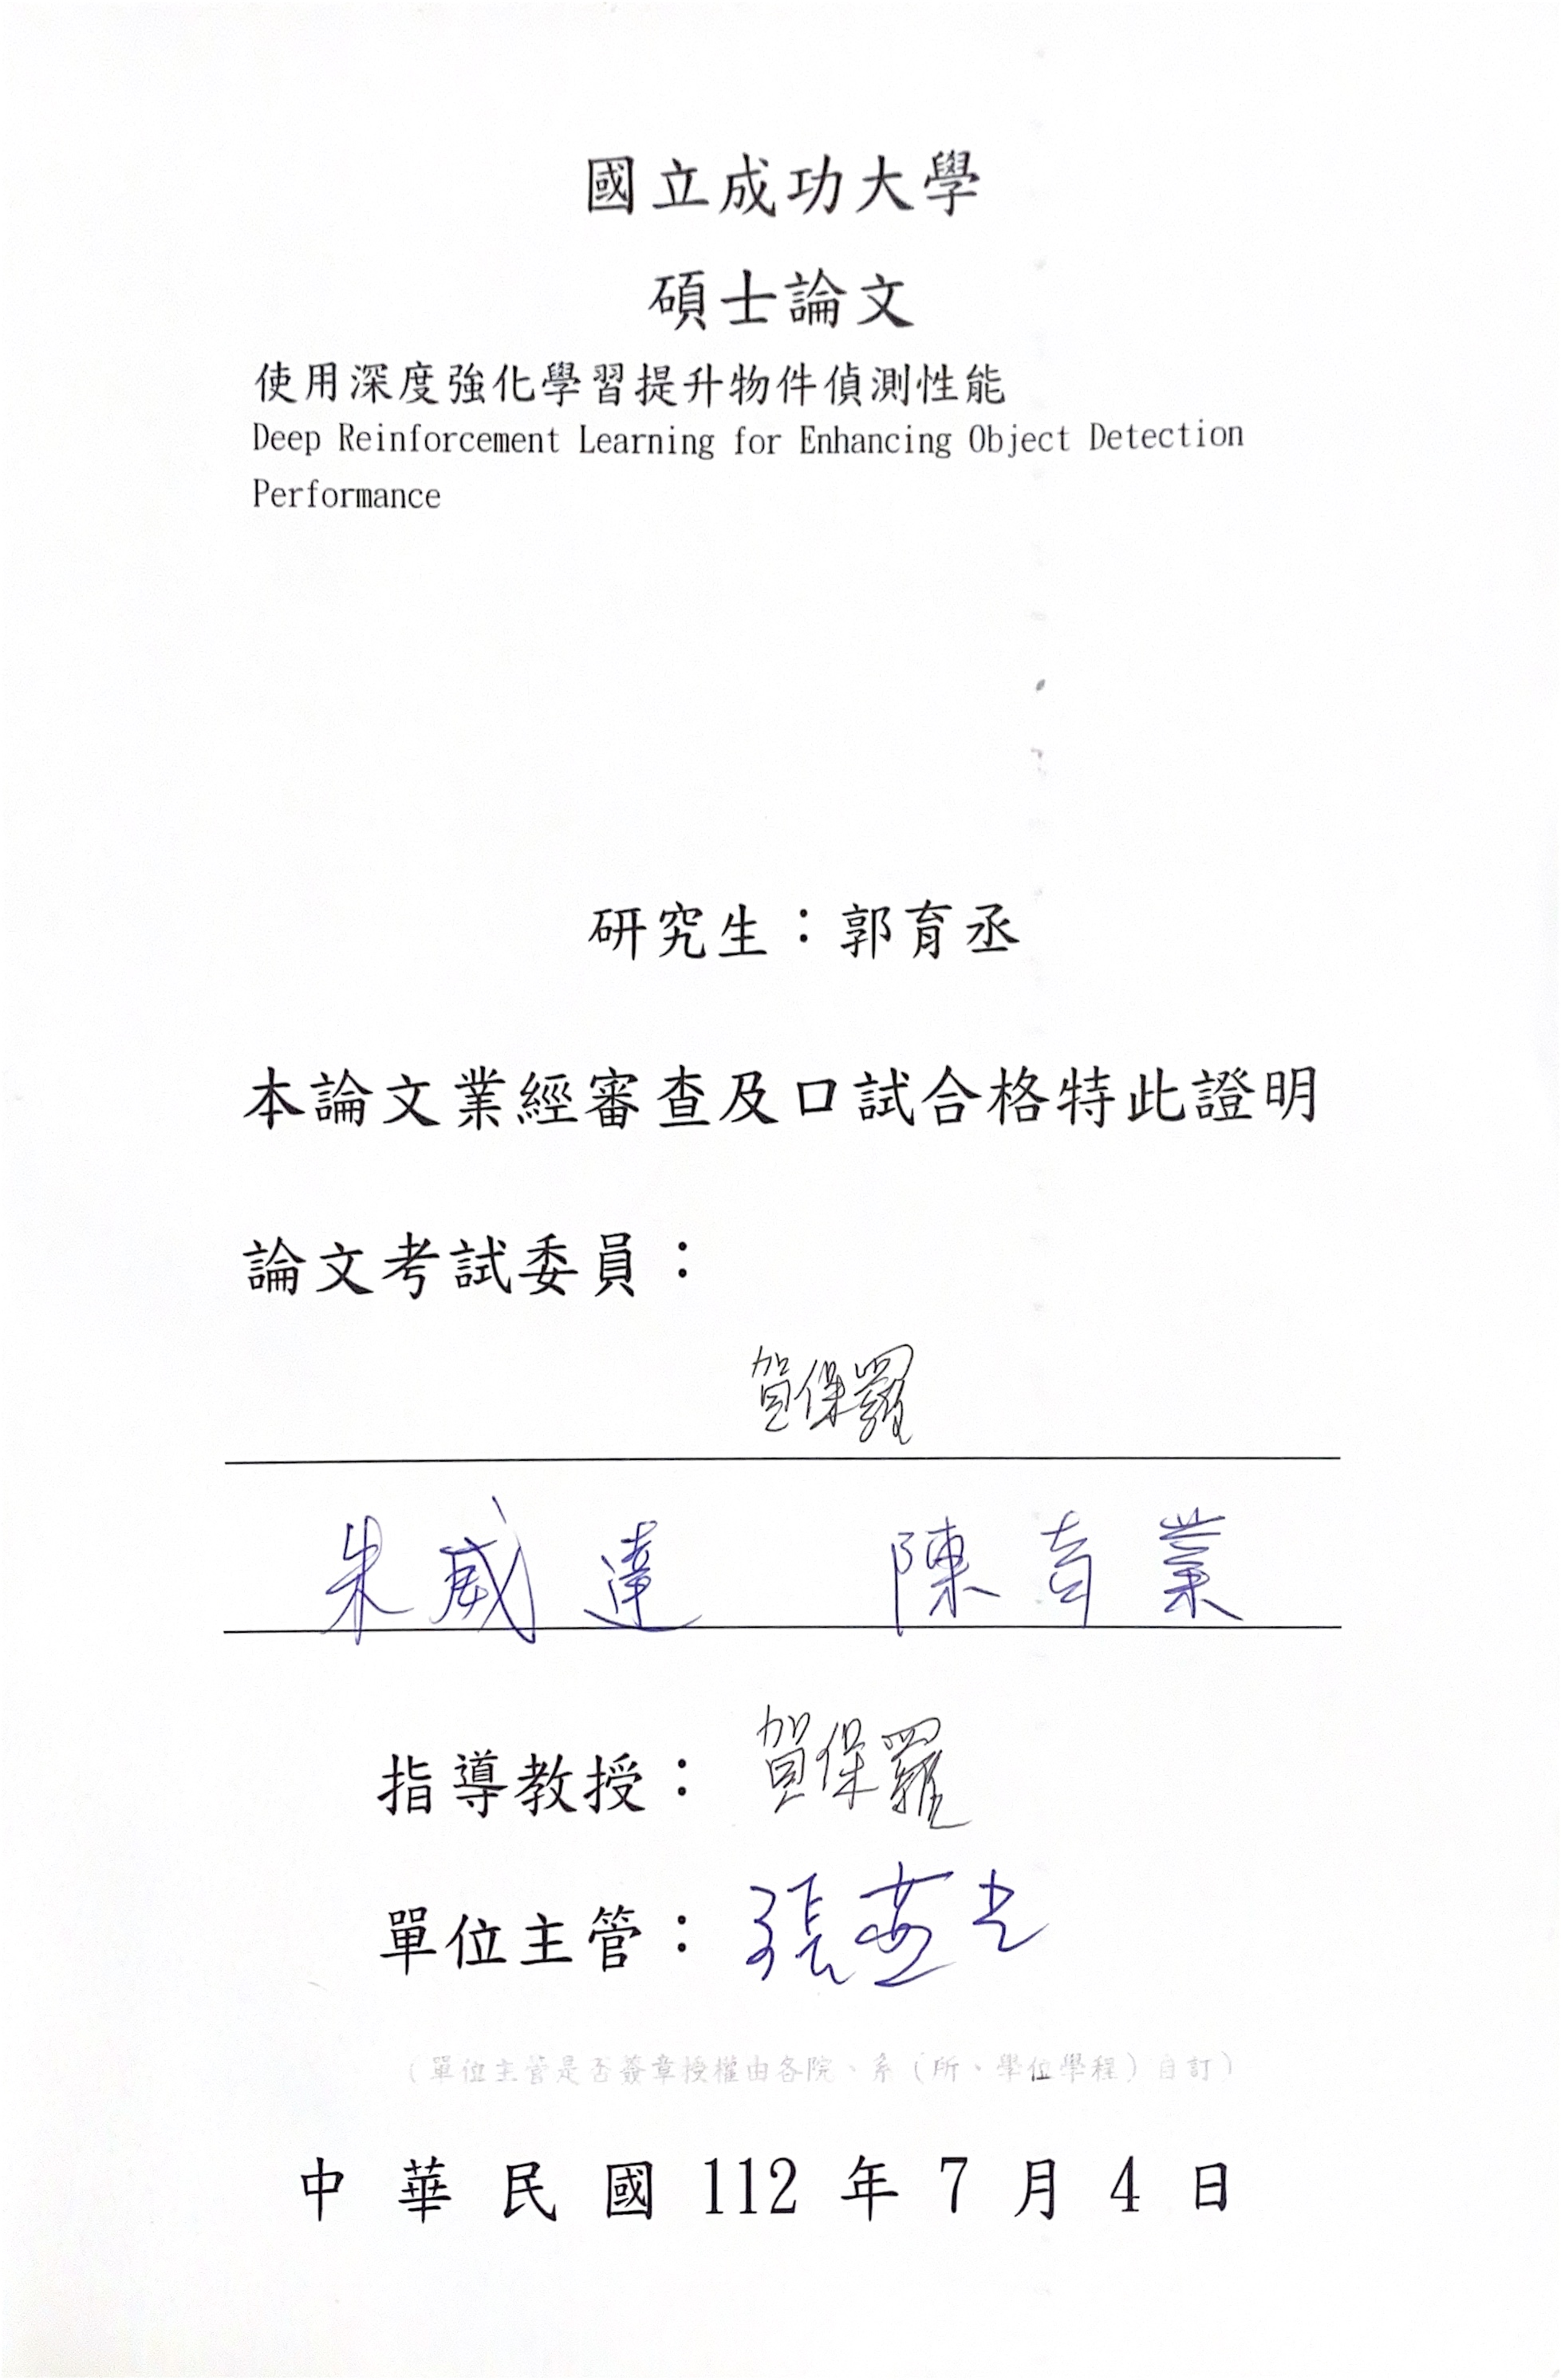
\includepdf{images/口試合格證明.pdf}

% 不會執行
\ifdefined\optCommittee
\newpage
\begin{center}
\vspace{1cm}
\SelectFontsizeBF{24}{%
\University中文\Department中文\\
\學位 論文}
\vfill
\SelectFontsizeBF{20}{\ThesisTitle中文}
\end{center}

\vfill
\SelectFontsize{20}{%
\noindent 研究生:\Student中文\\
本論文業經審查及口試合格特此證明}


\begin{center}
\SelectFontsize{18pt}{論文考試委員}
\vfill
\SignatureRule \hspace*{1cm} \SignatureRule
\vfill

\SignatureRule \hspace*{1cm} \SignatureRule
\vfill

指導教授:\SignatureRule[8]
\vfill
  所長:\SignatureRule[8]

\vfill
\SelectFontsize{18}{中華民國 \hspace{2em} 年 \hspace{2em} 月 \hspace{2em} 日}
\end{center}


\newpage
\begin{center}
\vspace{1cm}
\SelectFontsize{18}{\University英文, \Department英文}
\SelectFontsize{19}{\ifdef\PhD{Ph.D.}{Master's} Degree Thesis}

\vfill
\SelectFontsizeBF{20}{\ThesisTitle英文}
\end{center}

\vfill
\SelectFontsize{18}{Student: \Student英文}

\SelectFontsize{18}{%
A thesis submitted to the graduate division in partial fulfillment of the requirement for the degree of
\ifdef\PhD{Doctor of \mbox{Philosophy}}{Master of Science}.
}

\vfill
\begin{center}
\SelectFontsize{18}{Approved by}

\vfill
\SignatureRule \hspace*{1cm} \SignatureRule

\vfill
\SignatureRule \hspace*{1cm} \SignatureRule

\vfill
Advisor: \SignatureRule[8]

\vfill
Chairman: \SignatureRule[8]

\vfill
\SelectFontsize{18}{\YearMonth英文}
\vspace*{20pt}
\end{center}
\fi% optCommittee


\AddToContents{中文摘要}
\setcounter{page}{1}
\pagenumbering{roman}


\begin{center}
\SelectFontsizeBF{24}{\ThesisTitle中文}

\vspace{4mm}
\SelectFontsize{18}{\Student中文\footnote[1]{學生} ~ \Advisor中文\footnote[2]{指導教授}}

\vspace{5mm}
\SelectFontsize{20}{國立成功大學\Department中文}

\vspace{12mm}
\makebox[2.7cm][c]{\SelectFontsizeBF{22}{摘要}}
\end{center}

\vspace{4mm}
\SelectFontsize{16}{\Abstract中文}

\vspace{4mm}
\begin{flushleft}
\SelectFontsize{16}{\textbf{關鍵詞:} \Keywords中文}
\end{flushleft}



\AddToContents{Abstract}
\begin{center}
\SelectFontsizeBF{22}{\ThesisTitle英文}

\vspace{4mm}
\SelectFontsize{18}{\Student英文\footnote[1]{Student} ~ \Advisor英文\footnote[2]{Advisor}}

\vspace{4mm}
\SelectFontsize{16}{\Department英文, National Cheng Kung University}

\vspace{12mm}
\SelectFontsizeBF{20}{Abstract}
\end{center}

\vspace{4mm}
\SelectFontsize{14}{\Abstract英文}

\vspace{4mm}
\begin{flushleft}
\SelectFontsize{16}{\textbf{Keywords:} \Keywords英文}
\end{flushleft}



\AddToContents{誌謝}
\begin{center}\SelectFontsizeBF{24}{誌謝}\end{center}

\vspace{4mm}
\Acknowledgements



\renewcommand{\contentsname}{CONTENTS}
\AddToContents{Contents}
\tableofcontents


\AddToContents{List of Tables}
\listoftables


\AddToContents{List of Figures}
\listoffigures
% 封面頁, 口委中英文簽名單, 誌謝, 中英文摘要, 論文目錄, 圖表目錄


%────────────────────  List of Symbols  ────────────────────
% \renewcommand\nomgroup[1]{%
%   \item[\bfseries
%   \ifstrequal{#1}{A}{General}{%
%   \ifstrequal{#1}{Z}{Gene/Protein Names}%
%   }]}

% \nomenclature[A]{$\lg$}{Logarithm base 2}
% \nomenclature[A]{KL\ Divergence}{Kullback-Liebler Divergence}
% \nomenclature[Z]{Myc}{MYC proto-oncogene}
% \nomenclature[Z]{USF-1}{Upstream stimulatory factor 1}

% \printnomenclature[5cm]

\newpage
\setcounter{page}{1}
\pagenumbering{arabic}

\chapter{Introduction}
\section{Background}
In recent years, deep learning techniques have made remarkable advancements in various fields, particularly in the realm of image processing and analysis. Object detection, in particular, has gained significant attention due to its powerful recognition and localization capabilities, playing a critical role in numerous application scenarios. However, most deep learning models for object detection are trained on high-quality images, and their performance is heavily dependent on image quality. When images are affected by factors such as blurriness, noise, low contrast, inadequate lighting, or overexposure, the detection performance of these models may significantly degrade. Therefore, it becomes an important and challenging problem to enhance object detection accuracy under such non-ideal image conditions.

\section{Motivation}
Despite some existing research efforts to improve object detection performance under adverse image conditions by enhancing model structures or adjusting optimization strategies, these methods often require extensive parameter tuning and cannot guarantee satisfactory results in all situations. On the other hand, there has been limited exploration of using image preprocessing to improve image quality and, consequently, enhance object detection accuracy. Additionally, determining suitable preprocessing techniques and their corresponding parameters remains an unresolved challenge. Therefore, we believe that investigating the integration of deep learning and preprocessing techniques to improve object detection accuracy under adverse image conditions is a worthwhile research topic. To address this issue, we propose the use of Deep Deterministic Policy Gradient (DDPG), a deep reinforcement learning algorithm, to automatically determine the optimal image preprocessing strategy. The goal is to effectively enhance image quality and improve the accuracy of object detection.

\section{Objective}
The main contribution of this research is the first integration of deep reinforcement learning (DDPG) with the object detection model YOLOv7, applied in the image preprocessing stage to enhance object detection accuracy under adverse image conditions. Our approach considers image quality factors such as saturation, brightness, contrast, and sharpness, and employs deep reinforcement learning to automatically select the optimal preprocessing strategy for achieving the best image enhancement results. Through our experiments, we have demonstrated a significant improvement in object detection accuracy compared to using YOLOv7 alone. Our method not only enhances object detection performance but also provides a new direction for effectively handling image quality issues in deep learning.


\chapter{Materials and Related Works}
\section{Object Detection}
Object detection is an important topic in computer vision that aims to identify the location and classify specific objects in an image. Here is a review of some significant research in this field:

\subsection{Traditional methods}
Before deep learning became mainstream, some traditional methods for object detection have been widely studied and applied. For example, Histogram of Oriented Gradients (HOG) \cite{dalal2005histograms} and Deformable Part-based Model (DPM) \cite{felzenszwalb2009object} are two of the important methods.

The HOG algorithm performs object detection by analyzing the local shape information of an image. It first calculates the gradient direction and intensity of each pixel in the image and converts this information into a histogram representation. By counting the gradient direction in the local area, the HOG algorithm can capture the texture and shape features of the object. Combined with the support vector machine classifier, the extracted HOG features can be classified to achieve object identification and localization. 

The DPM algorithm treats an object as consisting of several deformable parts and learns the shape and appearance model of each part. It achieves more accurate detection and localization of objects by applying HOG features to each part of the object and establishing a constraint relationship between the parts. Similarly, DPM can be combined with a support vector machine classifier to achieve classification and identification of the extracted features.

% \begin{figure}[H]
%      \centering
%      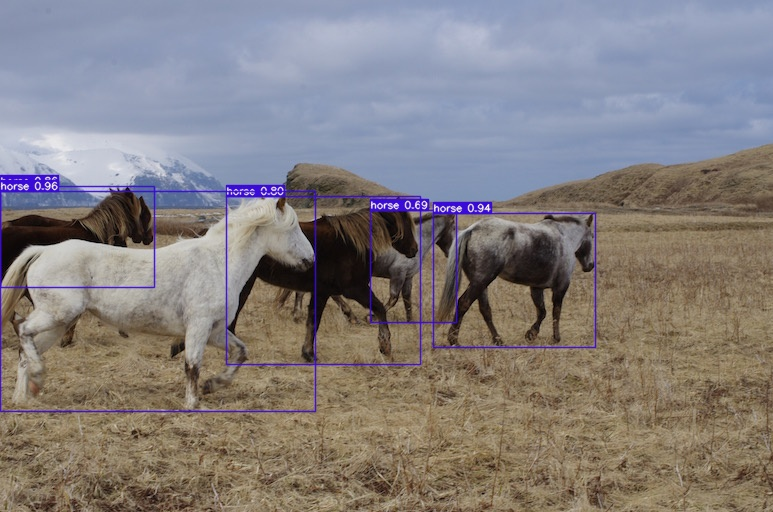
\includegraphics[width=0.5\textwidth]{images/object detective_example.jpg}
%      \caption{object detective} 
%      \label{Fig.Object detective} 
% \end{figure}

\subsection{Deep Learning methods}
With the rapid development of deep learning, a series of neural network-based object detection methods have been proposed. Girshick et al.~introduced R-CNN \cite{girshick2014rich}, a method that uses selective search to generate candidate regions and then performs feature extraction and classification using convolutional neural networks. Building upon R-CNN, Girshick and Ren et al.~further improved the efficiency and accuracy of object detection with Fast R-CNN \cite{girshick2015fast} and Faster R-CNN \cite{ren2015faster}, respectively.

Another significant research achievement is the YOLO \cite{redmon2016you} (You Only Look Once) series, which was introduced by Redmon et al. YOLO treats object detection as a regression problem and completes object identification and localization in a single inference pass. This approach not only enhances efficiency but also demonstrates excellent performance on various datasets. Multiple versions of YOLO (such as YOLOv2, YOLOv3, YOLOv4, etc.) have further improved the performance of the original model.

\textbf{You Only Look Once v7 (YOLOv7) \cite{wang2023yolov7}}: Compared with the previous state of the art YOLO series, YOLOv7 reduces the number of parameters by about 40\% and the amount of computation by about 50\% and is mainly divided into two aspects: model architecture optimization and training process optimization. For model architecture optimization, the authors propose extended and scaling methods to efficiently utilize parameters and computation; and for training process optimization, YOLOv7 uses re-parameterized and dynamic label assignment strategies, which can assign labels to different output layers more efficiently.

\begin{figure}[H]
    \centering 
    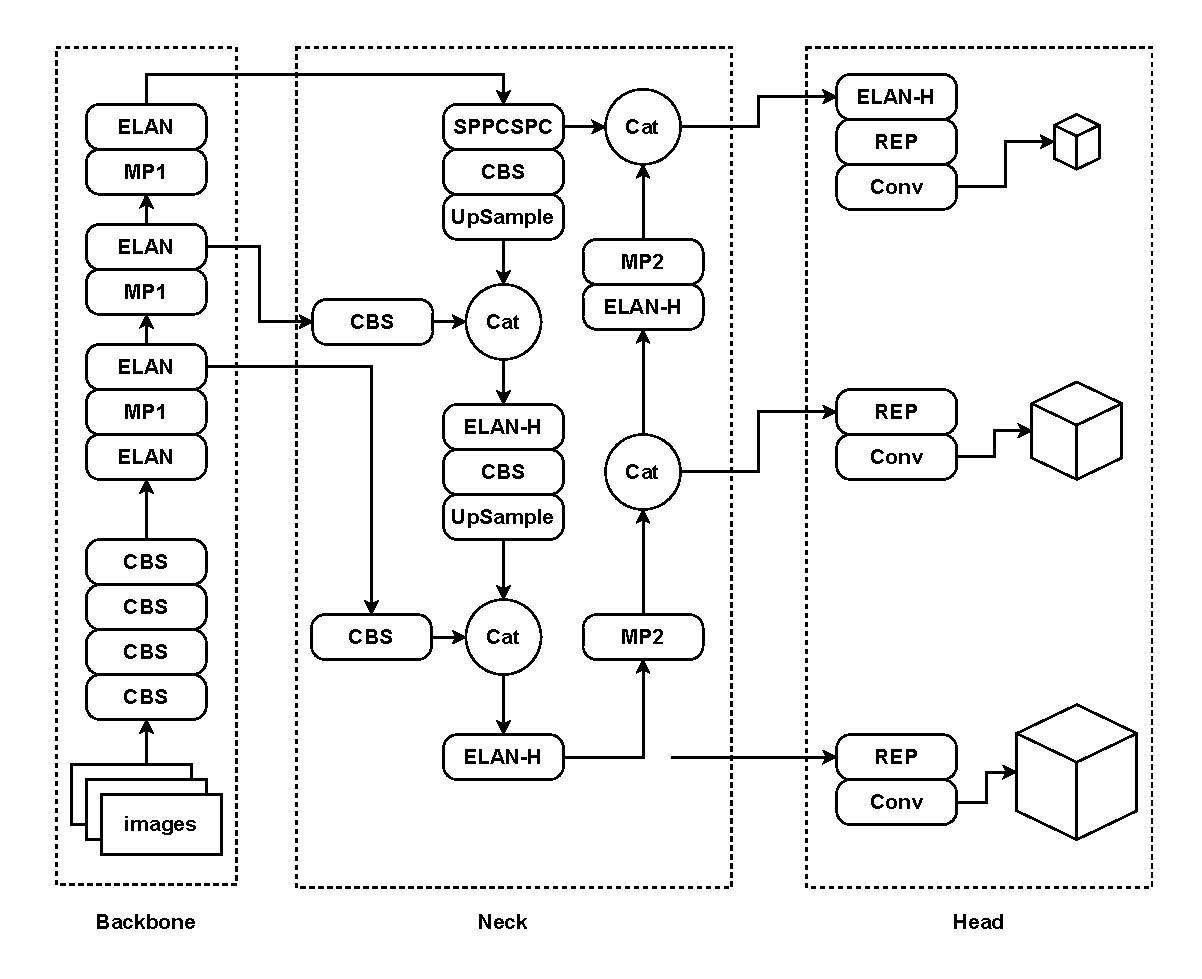
\includegraphics[width=0.9\textwidth]{images/YOLOv7 architecture.pdf}
    \caption{YOLOv7 architecture} 
    \label{Fig.YOLOv7 architecture} 
\end{figure}

In summary, research in the field of object detection has shifted from traditional methods to deep learning-based approaches, leading to significant advancements. However, despite the good performance of these methods in many scenarios, challenges still exist in handling complex backgrounds, small objects, and highly overlapping objects. Therefore, object detection remains an active research area that requires further study and development.

\section{Reinforcement Learning}
Reinforcement learning is a method in machine learning that enables models to learn and improve their behavior through interaction with an environment. In the framework of reinforcement learning, a agent takes actions to influence the environment and adjusts its behavior based on feedback from the environment, often referred to as rewards. The goal is to learn a policy that maximizes the accumulated rewards over time. Reinforcement learning has been successfully applied in various fields, including games, autonomous driving, robotics, natural language processing, and more.

\begin{figure}[H]
    \centering 
    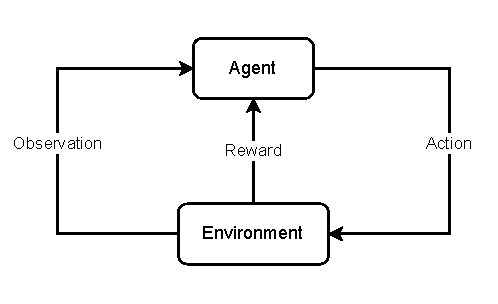
\includegraphics[width=0.8\textwidth]{images/RL architecture.pdf}
    \caption{Reinforcement learning architecture} 
    \label{Fig.Reinforcement learning architecture} 
\end{figure}

\textbf{Deep Deterministic Policy Gradient (DDPG) \cite{lillicrap2015continuous}}: A reinforcement learning algorithm widely used for problems in continuous action spaces. DDPG adopts an actor-critic architecture, which provides separate learning mechanisms for the actor and the critic, allowing for mutual improvement of the policy and value function. In DDPG, the actor is a policy function that aims to find a policy that maximizes the expected future rewards starting from the current state. The actor selects an action based on the current state, and this action influences the next state of the environment. The critic, on the other hand, is a value function that evaluates the goodness or badness of executing a certain action given a particular state. The critic's goal is to learn to predict the impact of the actor's policy on future rewards. The actor and the critic collaborate during the learning process. The actor improves its policy based on the feedback from the critic, while the critic improves its value function prediction based on the actor's policy. This combination enables DDPG to perform well in problems with continuous action spaces.

\begin{figure}[H]
    \centering 
    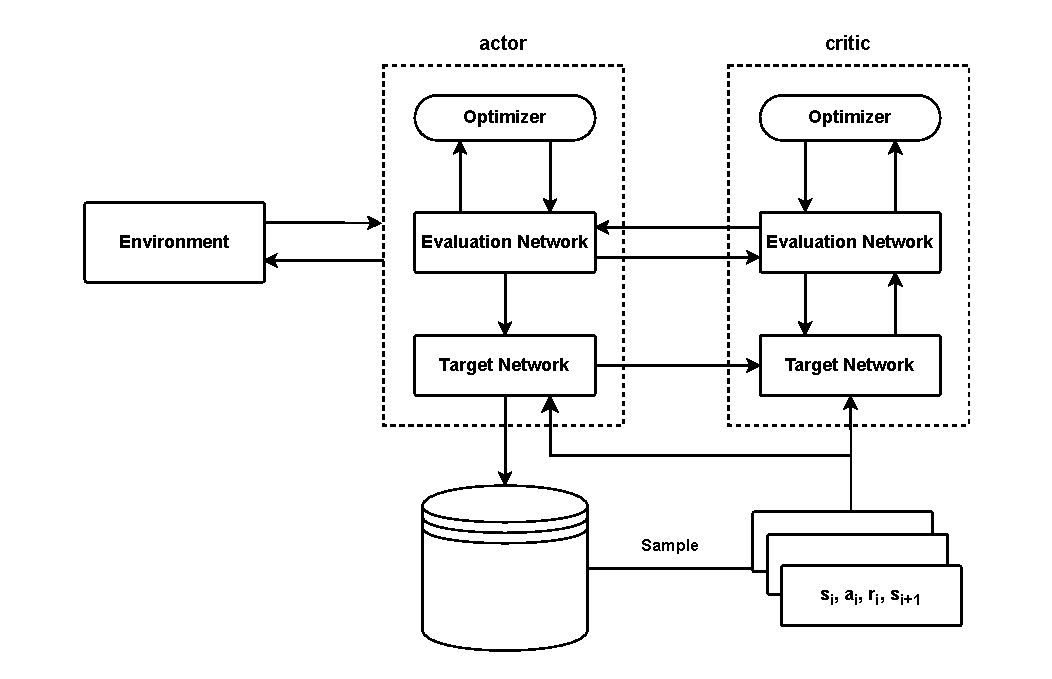
\includegraphics[width=\textwidth]{images/DDPG architecture.pdf}
    \caption{DDPG architecture} 
    \label{Fig.DDPG architecture} 
\end{figure}

\section{Related Works}
\cite{caicedo2015active}, \cite{bueno2017hierarchical} used DRL for object detection by treating the object detection problem as an MDP and using a hierarchical approach for object detection. In their approach, the Agent is responsible for finding the region of interest in the image and then finding smaller regions from the previously selected regions, thus forming the hierarchy. The authors consider several different actions to improve the accuracy of bounding boxes around the target. They use image feature vectors and action histories to represent states, and IOU transformations as a bonus.

\cite{jie2016tree} proposed an object detection method called Tree-RL, which utilizes two types of actions: panning (8 actions) and zooming (5 actions). The state is defined as the combination of the feature vector of the current window, the feature vector of the whole image, and the historical actions. Feature vectors are extracted from the ImageNet-trained VGG-16 model and rewarded with IOU transformations. tree-RL performs object detection by top-down tree search, starting from the whole image and selecting the best action in each window to generate two new windows.

\cite{nayak2020reinforcement} proposed a preprocessing algorithm called ObjectRL. The main idea is to adapt the preprocessing steps applied to the image so that the pre-trained object detector works more efficiently.The novelty of the ObjectRL algorithm is that it recognizes that an image that looks good to the human eye may not be suitable as an input to the pre-trained object detector. In other words, the subjective quality of an image may not be relevant to its object detection performance. Therefore, ObjectRL tries to select the most suitable image for the object detection task by learning appropriate preprocessing strategies. This work is similar to our work.


\chapter{Proposed Method}
\section{System Design}
The primary objective of this study is to improve the accuracy of object detection. We propose a method that combines Deep Deterministic Policy Gradient (DDPG) with YOLOv7 to enhance the effectiveness of object detection. This chapter will provide a detailed introduction to the system's design and implementation. Figure \ref{Fig.System workflow} shows the complete system flow chart.

\subsection{Preprocessing with DDPG}
In the entire system workflow, we first preprocess the image. This preprocessing stage involves using a technique called Deep Deterministic Policy Gradient (DDPG) to automatically adjust the image. Initially, we input the original image into the DDPG model. The DDPG model generates four parameters based on the image information, which are used to adjust the image's saturation, brightness, contrast, and sharpness. These parameters are known as transformation factors.

Next, we use these four transformation factors to adjust the original image and generate the adjusted image. This adjustment alters the visual characteristics of the image, enabling the subsequent object detection module to perform more accurate detections. Finally, we input the adjusted image into the YOLOv7 object detection model to enhance the accuracy of object detection.

During the model training process, we utilize the precision and recall of the image as the indicators derived from the output of the YOLOv7 model. These indicators are used to train the DDPG model, thereby enhancing the capabilities of DDPG. By continuously adjusting the transformation factors, the DDPG model learns how to generate better transformation parameters to optimize the performance of the object detection model.

After obtaining the four outputs from the DDPG model, we can adjust various aspects of the image including brightness, contrast, saturation, and sharpness through numerical methods. We provide a formula for adjusting the pixel intensity $(I)$ at the coordinate $(x,y)$. We assume that the transformation factor $\alpha$.

\begin{itemize}
\item \textbf{Brightness}: The brightness of an image can be changed by a factor $\alpha$ as follows:
\begin{equation}
I(x,y)=\min(\alpha\cdot I(x,y),255)
\end{equation}

\item \textbf{Contrast}: The contrast of an image can be changed by a factor $\alpha$ as follows: We define $gray()$ to convert an image into a grayscale image.
\begin{gather}
I_{gray}=\text{gray}(I)\notag \\
I(x,y)=\min(\alpha\cdot I(x,y)+(1-\alpha)\cdot\mathrm{mean}(I_{gray}),255)
\end{gather}

\item \textbf{Saturation}: The saturation of an image can be changed by a factor $\alpha$ as follows:
\begin{equation}
I(x,y)=\min(\alpha\cdot I(x,y)+(1-\alpha)\cdot I_{gray},255)
\end{equation}

\item \textbf{Sharpness}: The sharpness of an image can be changed by a factor $\alpha$ as follows: We define $blur()$ as blurring the image
\begin{gather}
I_{blur}=\text{blur}(I) \notag \\
I(x,y)=\min(\alpha\cdot I(x,y)+(1-\alpha)\cdot I_{blur},255)
\end{gather}
\end{itemize}

\subsection{Object Detective with Yolov7}
In the object detection module of the system, we use the pre-trained YOLOv7, an object detection model that can locate and classify objects simultaneously in a single inference. In this module, we take pre-processed images as input for object detection, and YOLOv7 analyzes and processes the images and outputs the results, including the object location and category. These outputs can be used to evaluate the performance of the object detection model, which we measure using two metrics: recall and precision.

Recall indicates the ability of the model to correctly detect the actual objects that are present, while precision indicates how many of the objects detected by the model are actually correct. The values of these metrics can be used for subsequent learning in the DDPG network.

\subsection{System Integration}
In the system, we integrate the preprocessing module and the object detection module, which improves the accuracy of object detection. The specific workflow is as follows: Firstly, the original image undergoes image adjustments through the preprocessing module. The preprocessing module utilizes the DDPG model to generate adjustment parameters based on the image information, and applies these parameters to the image, resulting in an adjusted image. The adjustment parameters include transformation factors for saturation, brightness, contrast, and sharpness.

Next, the adjusted image is inputted into the object detection module for object detection. The object detection module employs the YOLOv7 network for inference, and performs object localization and classification based on the image features. The output of the model includes the positions and class information of the detected objects.

In summary, in the entire system, we integrate the preprocessing module and the object detection module to enhance the accuracy of object detection. By adjusting the image through the preprocessing module and inputting the adjusted image into the object detection module, we can obtain more accurate object detection results. 

\begin{figure}[htb] 
\centering 
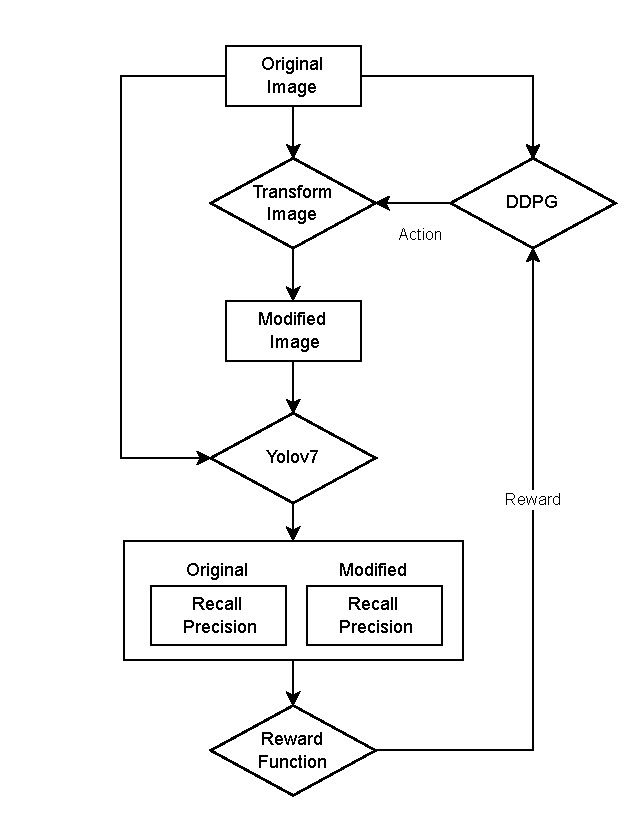
\includegraphics[width=\textwidth,height=\textheight,keepaspectratio]{images/system workflow.pdf}
\caption{System workflow} 
\label{Fig.System workflow} 
\end{figure}

\section{DRL Model}
In the following section, We will detail the deep reinforcement learning method we adopt, including the architecture of DDPG and the design principles of state, action, and reward.

\subsection{Network Archtecture}
Figure \ref{Fig.DDPG network architecture} is a network architecture diagram of DDPG, including the feature extraction network Resnet18 and the two-layer fully connected layer.

\begin{enumerate}[(i)]
\item \textbf{Feature Extraction Network - ResNet18}: \\
To extract important features from the input image, we utilize ResNet18 network. This is a deep residual network characterized by the inclusion of a large number of residual blocks in its architecture, effectively preventing the problem of gradient vanishing during training of deep networks. ResNet18 consists of 18 convolutional layers that process the input image through specific operations (such as batch normalization, ReLU activation, and residual connections), generating feature maps. These feature maps can be regarded as a high-dimensional representation of the input image, containing information about object shapes, textures, colors, and other details.

\item \textbf{Two Fully Connected Layers for Learning}: \\
After feature extraction through ResNet18, the generated feature maps are sent to two fully connected layers for further processing. The function of these fully connected layers is to learn useful features from the feature maps and make decisions. In our scenario, this decision involves adjusting the saturation, brightness, contrast, and sharpness of the image in order to improve the accuracy of object detection.
\end{enumerate}

\begin{figure}[H] 
    \centering 
    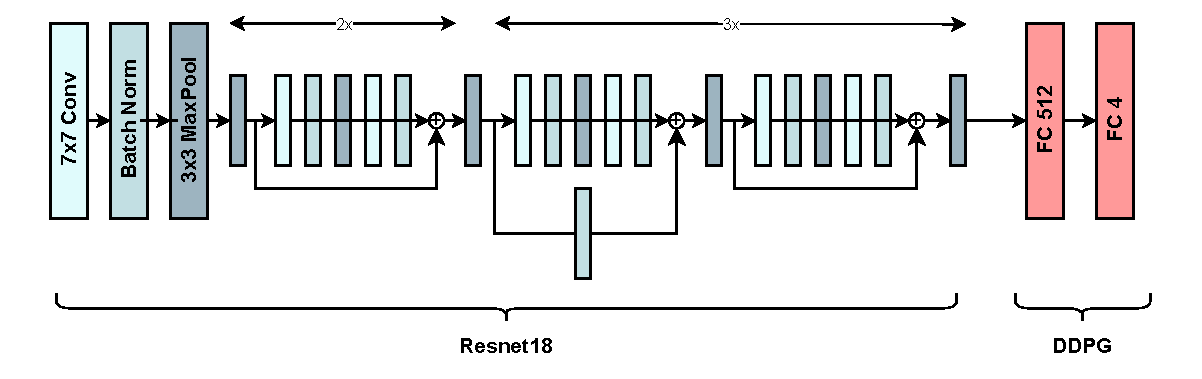
\includegraphics[width=\textwidth]{images/DDPG network architecture.pdf} 
    \caption{DDPG network architecture} 
    \label{Fig.DDPG network architecture} 
\end{figure}

\subsection{State}
The state of the agent is derived from RGB images from the COCO dataset \cite{lin2014microsoft}. Before inputting them into the DDPG model, the images are resized to a dimension of 224x224. This resizing step ensures uniformity in the input dimensions within the system for subsequent processing and analysis.

\subsection{Action}
The actions outputted by DDPG consist of four transformation factors: brightness, saturation, contrast, and sharpness. The values of these factors are constrained within the range of $a\in\lbrack0.5,1.5\rbrack$. By restricting the range of the transformation factors to 0.5 to 1.5, we ensure that the enhancement process does not result in excessive image distortion.

\subsection{Reward}
For an image inputted into YOLOv7, we evaluate the score using two metrics: the recall and the precision. By using the following formula, we can calculate the score of the image. We set $\alpha=0.5$.
\begin{equation}
S_i=\alpha\cdot({\mathrm{precision}}_i)+(1-\alpha)\cdot({\mathrm{recall}}_i)
\end{equation}
With the formula for calculating the score of an image, we can now present the complete formula for the reward function:
\begin{equation}
\label{reward function}
r_t={\beta\cdot\tanh(S_r-S_o)}
\end{equation}
In this formula, $S_r$ represents the score of the image after the action transformation, and $S_o$ represents the score of the original image. The difference between $S_r$ and $S_o$ indicates the variation in scores between the two images. A positive difference indicates that the adjusted image improves the detection performance of YOLOv7, while a negative difference suggests a negative impact on the detection performance. To ensure a smoother reward value, we use the $\tanh$ function. Additionally, the parameter $\beta$ is adjusted to control the curve of the $\tanh$ function, and in this case, $\beta$ is set to 4.0.


\chapter{Performance Evaluation}
In this section, we will introduce the content of the experiment, including the experimental design, experimental environment, and discuss the results of the experiment.

\section{Experimental Design}
In our experiment, we used the Coco dataset \cite{lin2014microsoft} as the training set. Due to the large size of the Coco dataset and limited experimental resources, we randomly sampled 20,000 data instances for training. A total of 10 epochs were conducted. Table \ref{Fig.DDPG parameter} presents the training parameters of DDPG.

During the training process, we primarily monitor changes in rewards. After training is completed, we proceed with testing. In our testing experiment, we utilize 5000 images, observing the score difference between the adjusted images and the original ones. Ultimately, we will compare the performance differences between object detection models preprocessed with DDPG and those without DDPG preprocessing. We will evaluate our results based on two key metrics: recall and precision.

\begin{table}[H]
	\centering
	\caption{DDPG Parameters}
        \label{Fig.DDPG parameter} 
	\begin{tabular}{p{5cm}p{5cm}}
		\toprule  %添加表格头部粗线
		\textbf{Parameter}   &\textbf{Value}  \\
		\midrule  %添加表格中横线
		\textbf{Episode}    & 10 \\
		\textbf{Replay buffer} & 4000   \\
		\textbf{batch size} & 32  \\
		\textbf{Actor network lr} & 0.003  \\
		\textbf{Critic network lr}   & 0.003 \\
		\textbf{Discount factor}   & 0.99 \\
		\textbf{Neurons per layer}   & 512, 4 \\
		\textbf{Optimizer}   & Adam \\
		\textbf{Activation function}   & ReLU \\
		\textbf{Loss function}   & MSE \\
		\bottomrule %添加表格底部粗线
	\end{tabular}
\end{table} 

\section{Experimental Result}
\subsection{DDPG Training Reward}
\begin{figure}[!htb] 
    \centering 
    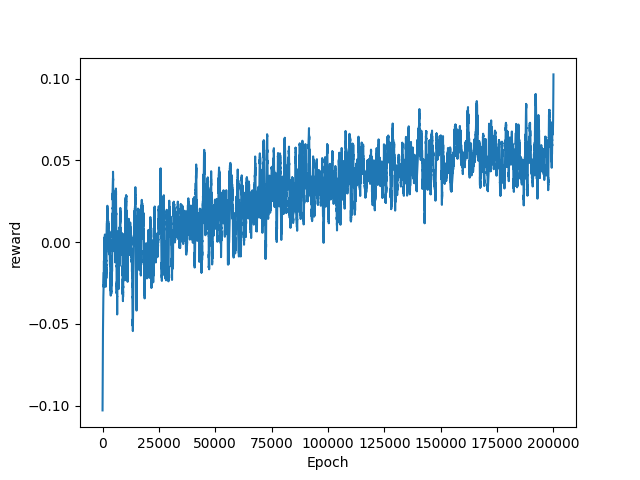
\includegraphics[width=0.9\textwidth]{images/training reward.png}
    \caption{Training reward} 
    \label{Fig.Training reward} 
\end{figure}
As shown in the figure \ref{Fig.Training reward}, after 10 epochs of training, our reward finally converged to 0.05. Our reward function is designed to easily generate so-called sparse rewards. In many images, the reward value is 0. There may be two reasons for this: one is that the objects in the image may have been completely detected, so no matter how the image is adjusted, its precision and recall will not increase, resulting in a reward of 0; another possible reason is that DDPG has not learned how to effectively adjust the image, thus getting the same detection result, and therefore the reward is 0. These two possible factors lead to a convergence of reward value at a lower level. However, although the reward seems to converge only to a relatively small value, it is still greater than 0, implying that DDPG has learned how to adjust the image to improve the effect of object detection.

\subsection{Test Score Differences with DDPG}

Among our 5,000 test images, more than 4000 images had a score difference of zero. This may suggest that in these images, DDPG's preprocessing did not change the result of object detection. For the remaining approximately 900 images, we observed a difference in scores, of which 691 images had a positive score difference, and 203 images had a negative score difference, as shown in Figure \ref{Fig./Test difference of score}.

A positive score difference implies that the image preprocessed by DDPG is superior to the original image in terms of object detection results, while a negative score difference means the detection effect is worse. However, we can see that among the images with a score difference, the number of images with a positive score difference is significantly more than the images with a negative score difference. This result indicates that using DDPG for preprocessing can improve the effect of object detection in some cases. However, we also noticed that for a portion of images (about 4\% of the test images), DDPG preprocessing may lead to a decrease in object detection efficiency. This could indicate that in certain special cases, the DDPG model has not yet found an appropriate preprocessing strategy.
\begin{figure}[!htb] 
    \centering 
    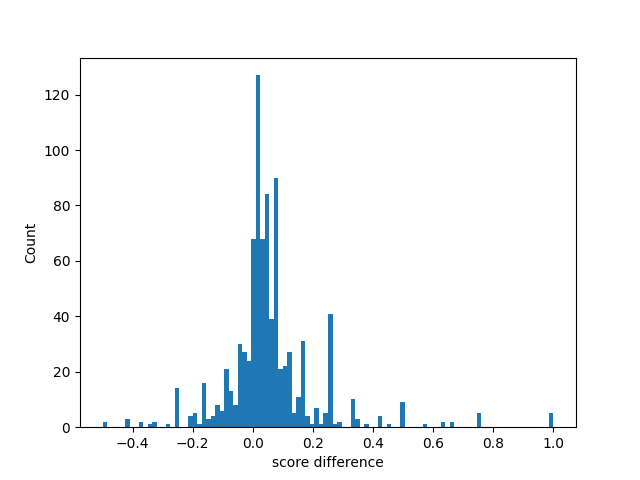
\includegraphics[width=0.9\textwidth]{images/test difference of score.png}
    \caption{Test difference of score} 
    \label{Fig./Test difference of score} 
\end{figure}

\subsection{DDPG Preprocessing in Object Detection: A Comparison}
To evaluate the impact of DDPG preprocessing on the performance of the object detection model, we separately compared the performance of the object detection models that used DDPG preprocessing and those that did not on the two main performance indicators: precision and recall. As shown in Figure \ref{Fig.Comparison result}, the object detection model processed by DDPG is 2.3\% higher in precision and 0.9\% higher in recall than the model not processed by DDPG.

These results show that DDPG preprocessing can improve the performance of object detection. Specifically, the improvement in precision means that our model's ability to predict correct objects has improved, reducing false positives. The improvement in recall implies that our model can more comprehensively identify objects in the image, reducing the occurrence of false negatives.
\begin{figure}[H] 
    \centering 
    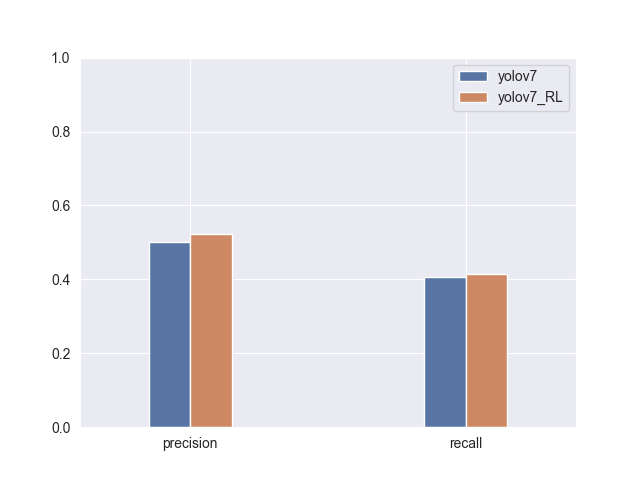
\includegraphics[width=\textwidth]{images/comparison result.png}
    \caption[Comparison Result]{Comparison of Object Detection Performance with and without DDPG Preprocessing} 
    \label{Fig.Comparison result} 
\end{figure}

\newpage
\section{Positive Instance}
\begin{figure}[H]
    \centering  %图片全局居中
    \subfigure{
    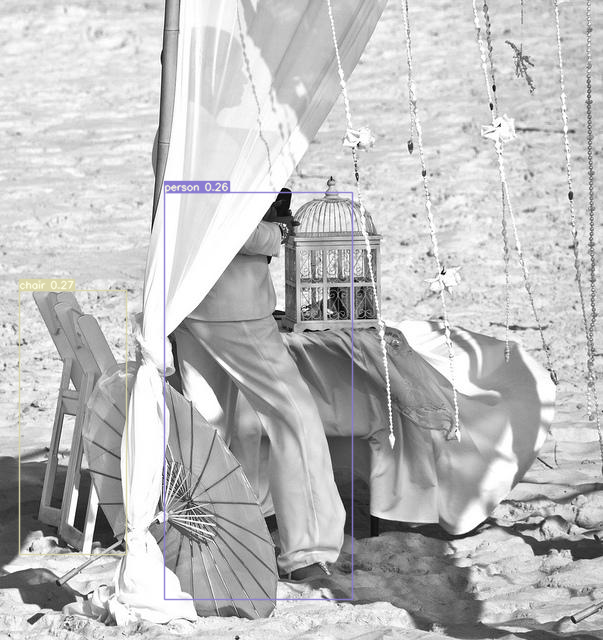
\includegraphics[width=0.45\textwidth]{images/instances/original_image_1.png}}
    \subfigure{
    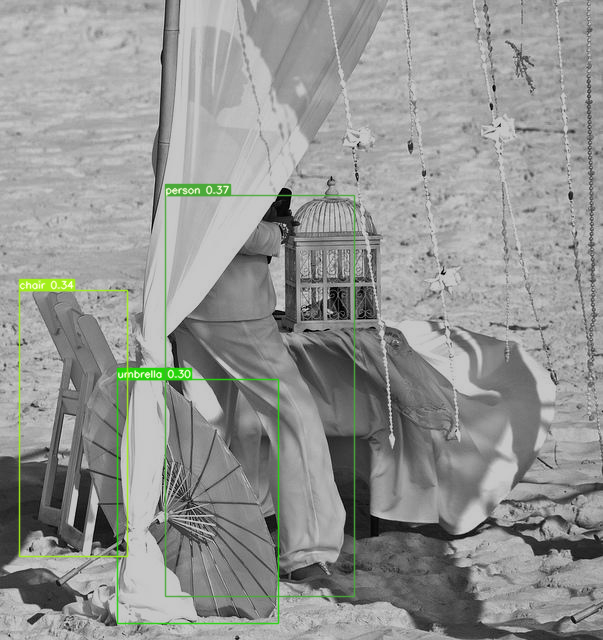
\includegraphics[width=0.45\textwidth]{images/instances/adjusted_image_1.png}}
    \setcounter{subfigure}{0}  %重新設置子圖計數器
    \subfigure[Original image]{
    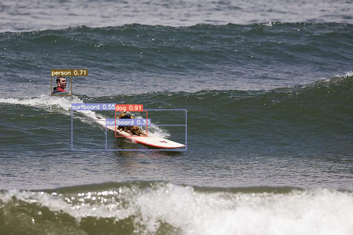
\includegraphics[width=0.45\textwidth]{images/instances/original_image_2.png}}
    \subfigure[Adjusted image]{
    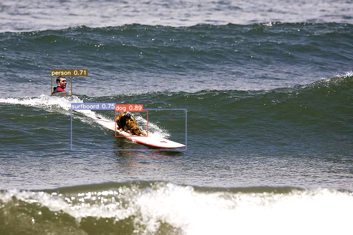
\includegraphics[width=0.45\textwidth]{images/instances/adjusted_image_2.png}}
    \caption[Positive instances with DDPG adjustments]{Positive instances that demonstrate the difference between the original images (left) and their DDPG-adjusted versions (right). It's noteworthy that objects that were not detected in the original images are successfully identified in the processed images.}
    \label{Fig.main}
\end{figure}

\chapter{Conclusion}
In this research, we proposed and tested a novel object detection method that combines deep reinforcement learning DDPG with the object detection model YOLOv7. Our results indicate that image preprocessing with DDPG can improve the precision and recall rates of object detection. However, this method might reduce detection effectiveness in some instances. Future studies should focus on further optimization of the DDPG model to cater to various image conditions. Additionally, our experiment was limited by the scale of our dataset, an issue we plan to address in future research by expanding our training and testing sets. Overall, our study provides a fresh perspective on improving the performance of object detection.

\newpage
\AddToContents{Bibliography}
\printbibliography


\end{document}
